%% modeloABNT2_Poli.tex, v1.0 monaro
%% Copyright 2015 by Athila e Monaro
%%
%% Este trabalho é uma adequação das normas de dissertações e teses
%% da Universidade de São Paulo - USP de acordo com a Norma ABNT
%%
%%
%% Quaisquer dúvidas favor enviar e-mail para:
%%
%% athila.uno@gmail.com ou
%% renato.monaro@gmail.com
%%

% ------------------------------------------------------------------------
% ------------------------------------------------------------------------
% eesc: Modelo de Trabalho Acadêmico (tese de doutorado, dissertação de
% mestrado e trabalhos monográficos em geral) em conformidade com 
% ABNT NBR 14724:2011. Esta classe estende as funcionalidades da classe
% abnTeX2 elaborada de forma a adequar os parâmetros exigidos pelas 
% normas USP e da Escola Politécnica.
% ------------------------------------------------------------------------
% ------------------------------------------------------------------------

% ------------------------------------------------------------------------
% Opções:
% 	tesedr:     Formata documento para tese de doutorado
%	qualidr:    Formata documento para qualificação de doutorado
% 	dissertmst: Formata documento para dissertação de mestrado
% 	qualimst:   Formata documento para qualificação de mestrado
%	tcc:     Formata documento para trabalho de conclusão de curso 
% ------------------------------------------------------------------------
%\documentclass[qualimst]{poli}
\documentclass[tcc]{poli}

% ---
% PACOTES
% ---

% ---
% Pacotes fundamentais 
% ---
\usepackage{cmap}				% Mapear caracteres especiais no PDF
\usepackage{lmodern}				% Usa a fonte Latin Modern			
\usepackage{makeidx}            	% Cria o indice
\usepackage{hyperref}  			% Controla a formação do índice
\usepackage{lastpage}			% Usado pela Ficha catalográfica
\usepackage{indentfirst}			% Indenta o primeiro parágrafo de cada seção.
\usepackage{nomencl} 			% Lista de simbolos
\usepackage{graphicx}			% Inclusão de gráficos
\usepackage{lscape}
\usepackage{amsmath}
\usepackage{multirow,makecell}

% ---

% ---
% Pacotes adicionais, usados apenas no âmbito do Modelo eesc
% ---
\usepackage{lipsum}				       % para geração de dummy text
\usepackage[printonlyused]{acronym}
\usepackage[table]{xcolor}
% ---
% Pacotes fusco
% ---
\usepackage{listings}
\usepackage{color}
\definecolor{lightgray}{rgb}{.9,.9,.9}
\definecolor{salmon}{rgb}{1,0.5,0.3}
\definecolor{purple}{rgb}{0.65, 0.12, 0.82}

\lstdefinelanguage{JavaScript}{
  keywords={typeof, new, true, false, catch, function, return, null, switch, var, const, if, of, in, while, else, case, break},
  keywordstyle=\color{blue}\bfseries,
  ndkeywords={class, export, boolean, throw, implements, import, this, require, then, pipe, log, setTimeout, write, catch},
  ndkeywordstyle=\color{salmon}\bfseries,
  identifierstyle=\color{black},
  sensitive=false,
  comment=[l]{//},
  morecomment=[s]{/*}{*/},
  commentstyle=\color{purple}\ttfamily,
  stringstyle=\color{red}\ttfamily,
  morestring=[b]',
  morestring=[b]"
}


\lstdefinestyle{code}{
   language=JavaScript,
   backgroundcolor=\color{lightgray},
   extendedchars=true,
   basicstyle=\footnotesize\ttfamily,
   showstringspaces=false,
   showspaces=false,
   numbers=left,
   numberstyle=\footnotesize,
   numbersep=9pt,
   tabsize=2,
   breaklines=true,
   showtabs=false,
   captionpos=b
}

\lstset{
   style=code
}

% ---
% Informações de dados para CAPA e FOLHA DE ROSTO
% ---
%
% Título:
%	1. Título em português
%	2. Título em inglês
\titulo{Análise da receita potencial de arbitragem utilizando sistemas de armazenamento de energia elétrica em mercados de energia}{Analysis of the potential arbitrage income using electricity storage system in energy markets}
%
% Autor:
%	1. Nome completo do autor
%	2. Formato de nome para bibliografia
\autor{Lucas Marquez Tonim

Luis Felipe Viveiros Fusco} {Tonim, L. M.; Fusco, L. F. V.}
%

% Cidade
\local{São Paulo}
% Ano de defesa
\data{2019}

% ---
% Inserir Área de concentração
%
% O comando \areaconcentracao deve ser definido apenas para documentos de pós-graduação.
% Caso contrário deve-se considerar a necessidade do comando \enfase
%\areaconcentracao{Sistemas Elétricos de Potência}
% ---
%
% O comando \enfase deve ser definido apenas para documentos de TCC.
% Caso o aluno tenha cursado os créditos necessários
\enfase{Energia e Automação Elétricas}
%
% CUIDADO: Apenas um das opç?es acima deve ser escolhida para o documento
% ---


% Nome do orientador
\orientador{Prof. Dr. Maurício Barbosa de Camargo Salles}
% Nome do coorientador
%\coorientador{Coorientador}
% ---

% ---
% compila o indice
% ---
\makeindex
% ---

% ---
% Compila a lista de abreviaturas e siglas
% ---
\makenomenclature
% ---
% ---
% Inserir ficha catalográfica
%
% Caso o comando \inserirfichacatalografica seja definido, a ficha catalográfica
% será inserida atrás da folha de rosto. Caso contrário a página será deixada em
% branco.
%
% CUIDADO: Esta opção deve ser preenchida antes do comando \maketitle
% ---
\inserirfichacatalografica{EPUSP-Catalogacao-na-Fonte.pdf}
% ---

% ---
% Inserir folha de aprovação
%
% Caso o comando \inserirfolhaaprovacao seja definido, a a folha de aprovação
% será inserida. Além disso, conforme Resolução CoPGr 5890, as informações 
% de rodapé são inseridas apropriadamente na folha de rosto.
%
% CUIDADO: Esta opção deve ser preenchida antes do comando \maketitle
% ---
%%%%%%%%%%%%%\inserirfolhaaprovacao{folhaAprovacao.pdf}
% ---

% ----
% Início do documento
% ----

\begin{document}

% ----------------------------------------------------------
% ELEMENTOS PRÉ-TEXTUAIS
% ----------------------------------------------------------
\pretextual
% ---
% Insere Capa, Folha de rosto, Ficha catalográfica (se inserida)
% e folha de aprovação (se inserida).
% ---
\maketitle
% ---
% Dedicatória
% ---
%\imprimirdedicatoria{
%Este trabalho é dedicado a nossas famílias.
%}
% ---
% ---
% Agradecimentos
% ---
%\imprimiragradecimentos{
%Agradecimentos.
%}
% ---

% ---
% Epígrafe
% ---
%\imprimirepigrafe{
%}
% ---

% ---
% RESUMO e ABSTRACT
% ---

% Resumo em português

\begin{resumo}{palavras chaves. eng eletrica. mercado livre. PJM. BESS. otimização. AMPL}
%
O constante desenvolvimento do mercado livre brasileiro de energia através de novas legislações, traz novidades para o mercado nacional que já estão melhor fundamentadas em alguns mercados estrangeiros. Como é o caso da precificação da energia elétrica em base horária, algo que já é realidade no mercado norte-americano PJM e que há previsão de chegar ao Brasil em meados de 2020. Este estudo propõe operar um sistema de armazenamento de energia elétrica à baterias de íons de lítio. O sistema será modelado considerando o envelhecimento das baterias. O objetivo é chegar a conclusões sobre a viabilidade econômica de praticar a arbitragem de energia considerando as condições de operação do sistema. Para tanto, serão adquiridos os preços da energia elétrica do mercado PJM em base horária, será feita a modelagem do envelhecimento da bateria na linguagem AMPL e por fim os dados serão consolidados num plataforma de \textit{business analytics}.

\end{resumo}

% Resumo em inglês

\begin{abstract}{key words. electrical eng. energy market. PJM. BESS. optimization. AMPL}
%
The constant development of the Brazilian free energy market through new legislations, brings news to the national market that are already consolidate in some foreign markets. As the case with hourly priced electricity, something that is already a reality in the USA PJM market and that is expected to arrive in Brazil by 2020. This study proposes to operate a lithium-ion battery energy storage system on the PJM market. The system will be modeled considering the aging of the batteries. The objective is to come to conclusions about the monetary feasibility considering this operation as an investment. In order to achieve this, the electric energy prices of the PJM market will be acquired on an hourly basis, the aging of the battery will be modeled in the AMPL language and finally the data will be consolidated in a business analytics platform.
%
\end{abstract}
% ---

% ---
% inserir lista de ilustrações
% ---
\listailustracoes
% ---

% ---
% inserir lista de tabelas
% ---
%\listatabelas
% ---
% ---
% inserir lista de abreviaturas e siglas
% ---
\listasiglas{abrev/Abreviaturas}
% ---
% ---
% inserir o sumario
% ---
\sumario
% ---

% ----------------------------------------------------------
% ELEMENTOS TEXTUAIS
% ----------------------------------------------------------
\mainmatter

% ----------------------------------------------------------
% Introdução
% ----------------------------------------------------------
\chapter[Introdução]{Introdução}
\label{intro}

O mercado livre de energia no Brasil vem crescendo e amadurecendo ao longo do tempo. Em seus mais de 20 anos de existência, passou por importantes avanços de legislação visando disponibilizar fontes de geração cada vez mais limpas, distribuídas e seguras além de garantir a liberdade de negociação ao consumidor \cite{folha2018ml}. 

Entre as propostas legislativas, é possível identificar algumas aproximações com o mercado norte-americano de energia elétrica \cite{ccee2018}. Atualmente no Brasil, o \ac{PLD} é calculado em uma base semanal pela \ac{CCEE} e é regulamentado pela \ac{ANEEL}. 

Já nos Estados Unidos, em algumas regiões, esse cálculo é feito e disponibilizado em um ritmo muito mais intenso; em mercados como o PJM, o cálculo da tarifa do tipo \textit{Real-Time} é feito a cada 5 minutos \cite{pjmEnergyMarket}. A partir disso, surge um mercado muito mais competitivo e que exige um certo conhecimento e estudo prévio além do desenvolvimento de modelos e algoritmos de cálculos para que as tomadas de decisão nesse novo mercado muito mais veloz sejam bem embasadas.

O PJM é um mercado competitivo e atacadista que gerencia a confiabilidade de sua rede de transmissão, despachando e coordenando o fluxo de potência em sua zona de atuação. Esse mercado inclui a negociação do Mercado do Dia Seguinte ou \ac{DAM} e Mercado em Tempo Real ou \ac{RTM}, armazenamento e serviços auxiliares. \cite{fercPJM}

Traçando um paralelo com o mercado brasileiro, é possível identificar que o mercado norte-americano possui características que estão vindo gradualmente para o país, como, por exemplo, a negociação em tempo real através do cálculo horário da tarifa. Assim, é de grande importância para o mercado livre nacional a assimilação de algoritmos de cálculos baseados em nós da rede e em regime horário de operação e das estratégias de negociação decorrentes.

\section{Objetivos}

Compreender o mercado de energia norte-americano com enfoque no PJM e suas especificidades, como o cálculo do \ac{LMP} que por sua vez reflete diretamente no preço praticado da energia, entendimento de conceitos como \textit{Real-Time Pricing} (Precificação em Tempo Real), \textit{Day-Ahead Market} (Mercado do Dia Seguinte) e o impacto desses fatores no traçado de estratégias de compra, venda e estocagem de energia elétrica para maximização da receita. 

Adotar e implementar na linguagem de programação algébrica AMPL modelos matemáticos que correspondam à baterias de lítio levando em conta seu envelhecimento e desgaste de modo a aperfeiçoar o algoritmo que usava um modelo genérico visto em \cite{salles2017}. 

Finalmente, será feita uma análise dos conjunto de dados obtidos em uma plataforma de \textit{Business Analytics} e os dados serão dispostos de maneira interativa e simplificada para fácil acesso a possíveis investidores e interessados na área. 









% ----------------------------------------------------------
%Desenvolvimento
% ----------------------------------------------------------
\chapter[Metodologia e Desenvolvimento]{Metodologia e Desenvolvimento}
\label{metodologia}

\section{Conceitos e detalhes do PJM, um mercado livre de energia}
O PJM é um \ac{RTO} e um \ac{ISO}, responsável por coordenar e fazer a gestão do maior mercado atacadista de energia mundial. Esses status foram conseguidos ao longo do tempo, com a autorização da \ac{FERC}, agência americana que regula a transmissão de energia interestadual. Em 2018, conforme citado no relatório anual \cite{2018_anual_report}, o mercado possuia uma capacidade de geração de 180 086 MW e movimentou 805 546 GWh, o equivalente a U\$49,80 bilhões. Ele atende 65 milhões de pessoas, em um território de 593 989 $km^{2}$ (369 089 milhas quadradas), composto por 13 estados (Delaware, Illinois, Indiana, Kentucky, Maryland, Michigan, Nova Jersey, Carolina do Norte, Ohio, Pensilvânia, Tennessee, Virgínia, Virgínia Ocidental), além do Distrito de Colúmbia e é composto por 135 564 Km (84 236 milhas) de linhas de transmissão. 

O nome PJM é oriundo do nome das concessionárias dos três estados formadores (\textbf{P}ensilvânia, Nova \textbf{J}ersey, \textbf{M}aryland), que teve início em 1927. Desde então, ele vem aprofundando cada vez mais a sua área de ocupação, além das atividades desempenhadas. Hoje, ele opera de maneira independente e neutra a fim de garantir a confiabilidade e segurança da rede, além de criar um ambiente competitivo e integrado entre os seus membros (Geradores, Transmissores, Distribuidores e Consumidores), permitindo o acesso a energia a um baixo custo.

%% FIGURA 1 - Zonas
\begin{figure}[htb]
	\caption{Zonas do PJM.}
	\begin{center}
	    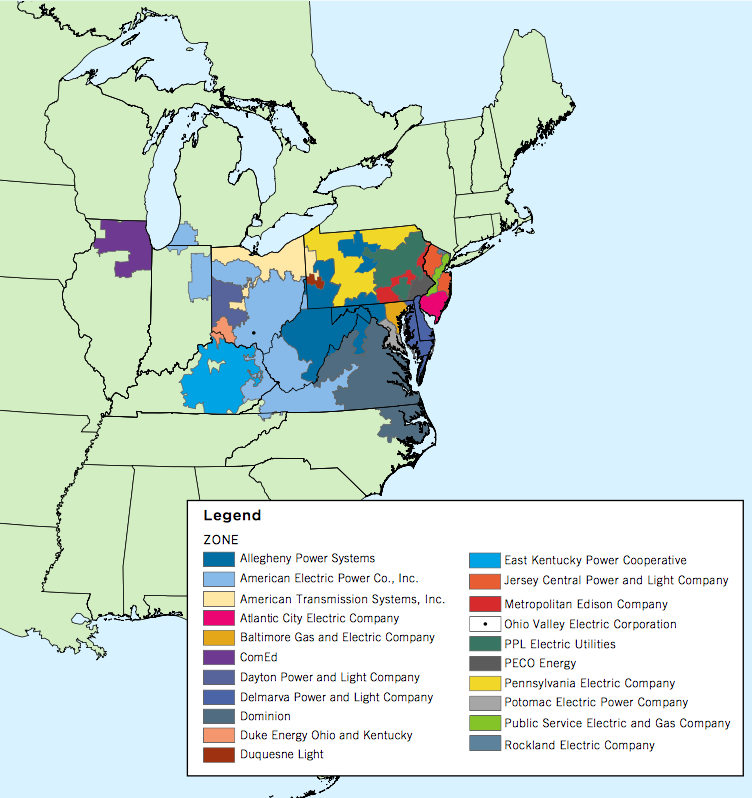
\includegraphics[scale=.5]{figuras/Zonas_PJM.png}
	\end{center}
   \begin{center}
      \footnotesize {Fonte: \cite{Zonas}}
   \end{center}
    \label{fig:Zonas}
\end{figure}

%% FIGURA 2 - Zonas
\begin{figure}[htb]
	\caption{Malha do PJM.}
	\begin{center}
	    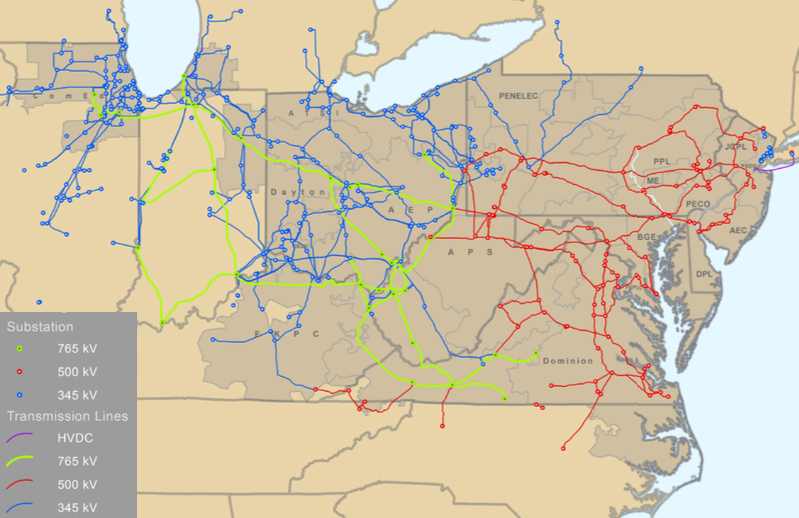
\includegraphics[scale=.5]{figuras/Malha_PJM.png}
	\end{center}
   \begin{center}
      \footnotesize {Fonte: \cite{Malha}}
   \end{center}
    \label{fig:Malha}
\end{figure} 

O PJM permite a comercialização de energia através de contratos bilaterais, em que as partes definem os termos da negociação ou organizado pelo mercado atacadista, o qual é regulamentado pela \ac{FERC}, e tem sua negociação através de seus submercados de energia: \ac{DAM} e \ac{RTM}. 
Em ambos os mercados de energia o preço da energia comercializada varia de acordo com o nó, ou seja, da localização no sistema, assim como pode variar de hora em hora. Isso acontece pois a definição do preço da energia, ou seja, o \ac{LMP} é calculado de forma dinâmica, porém seu cálculo varia um pouco de um submercado para outro, apesar de possuírem a mesma essência. A negociação nesses submercados ocorre de maneira similar a de um leilão, em que o negócio só se concretiza quando a oferta do consumidor (preço e potência em determinado horário) é atendida pela oferta de um gerador (preço e potência em determinado horário).
%\bigskip

\subsection{\textit{Locational Marginal Price} (LMP)}

%\medskip
É o método utilizado pelo PJM para precificar energia comercializada em um determinado nó, para um determinado horário, em cada submercado de energia e ele, o \ac{LMP} é o valor pago pelo consumidor ao gerador. Por conta desta peculiaridade um nó no \ac{DAM} pode ter um \ac{LMP} diferente do \ac{LMP} no \ac{RTM} para um mesmo nó em um mesmo momento do dia, porém ambos são definidos a partir da soma de três variáveis, as quais são calculadas independentemente uma da outra. São elas:
    \begin{itemize}
        \item \textit{System Energy Price}:
É calculado baseado no despacho ótimo, ignorando o congestionamento da rede e as perdas de energia na transmissão. 
Esta componente do \ac{LMP} apresenta o mesmo valor para todos os nós do PJM.

		\item \textit{Transmission Congestion Cost}:
		Representa o preço do congestionamento da rede em decorrência das restrições na ligação entre o gerador e o consumidor, por isso pode variar de nó para nó. Pode ter valor negativo, quando o nó está na zona descongestionada (baixas restrições) e valores positivos na parte mais congestionada (altas restrições) da rede. Seu valor é zero quando não há restrições. Essas restrições são provenientes dos limites térmicos, tensão máxima e limite de estabilidade do sistema de transmissão. O Gerador recebe e a carga paga esta variável referente ao \textit{Congestion Price}.

		\item \textit{Cost of Marginal Losses}:
		Representa o preço das perdas nas linhas de transmissão ocorridas entre o gerador e o consumidor. Esta variável representa o aumento das perdas ao aumentar pouco a injeção ou consumo de energia na rede. Assim como o \textit{Transmission Congestion Cost}, ele pode variar de nó para nó, é pago pela carga e recebido pelo gerador, além de poder apresentar valor negativo. Se o gerador está próximo da carga, o \textit{Cost of Marginal Losses} é positivo, caso o gerador esteja longe da carga, ele apresenta valor negativo.
    \end{itemize}

Os custos que variam de nó para nó são importantíssimos, pois eles acabam dando um direcionamento na localização de novos geradores, de modo que estejam perto dos consumidores para que o mercado possa ser mais eficiente e ter valores otimizados de \textit{Transmission Congestion Cost} e de \textit{Cost of Marginal Losses}.

%\bigskip
    
\subsection{Mercado de Energia - \textit{Day-Ahead} (DAM)} 
   %\medskip
        
Este é um mercado futuro de curto prazo, pois o preço da energia de todos os horários do dia seguinte são pré-definidos no dia anterior. Entre as 16h e 18h do dia anterior, os geradores e consumidores devem fazer suas ofertas com preço e energia para cada horário do dia. As ofertas são feitas de forma anônima e processadas pelo do PJM, que calcula o \ac{LMP} (preço da energia) para cada horário no dia seguinte, a fim de ter menores perdas e congestionamento da rede ao conectar o gerador ao consumidor. Nesta etapa também é definido o quanto o gerador e o consumidor terão direito no \ac{DAM}, pois caso haja diferença (excedente ou falta) eles precisarão comercializar no mercado Real-Time. O cálculo do \ac{LMP} para o \ac{DAM} já leva em consideração o custo de congestionamento da rede, assim como confiabilidade e reservas de energia obrigatórias estimadas para o \ac{RTM}.  Por conta de ter o preço fixado com antecedência e todos os parâmetros terem sido calculados com base no fluxo de energia declarado pelas parte, tanto o gerador quanto o consumidor tem o compromisso de  exercer o que foi pré-determinado pelo PJM. Caso haja falta ou excesso da oferta que foi feita em relação ao determinado pelo PJM, o gerador ou consumidor deverá operar no \ac{RTM}. No \ac{DAM}, também são definidos os \textit{Financial Transmission Rights} (FTRs).

%\bigskip
    

\subsection{Mercado de Energia - \textit{Real-Time} (RTM)}
%\medskip

Este é o mercado instantâneo de energia. O \ac{LMP} é calculado a cada 5 minutos pelo \textit{Locational Price Algorithm} (LPA), de acordo com os parâmetros instantâneos da rede, valores que são agregados e definem o \ac{LMP} da hora do \ac{RTM}. Neste mercado, operam principalmente os consumidores e geradores que não conseguiram despachar ou comprar a energia desejada no \ac{DAM}, porém os preços praticados são o do \ac{RTM}. O PJM faz uma gestão ativa e instantânea da rede, de modo a cada 5 minutos enviar sinais eletrônicos para informar aos consumidores e geradores a oferta de energia deles nos próximos 5 minutos. O monitoramento do congestionamento da rede também é feito a todo instante, a fim de manter a segurança e confiabilidade da rede. Em situações extremas, o PJM chega a dar incentivos a geradores para que produzam mais energia, assim como incentivos a consumidores para que reduzam o consumo momentâneo, tudo para manter os padrões de segurança e confiabilidade.

%\bigskip
Por conta de toda esta complexidade e dinamicidade para manter a confiabilidade e segurança da rede elétrica, monitora as redes, faz simulações diversas, que estressam desde condições climáticas, falha de diversos equipamentos, além de situações emergenciais e de estar sempre se reinventando e buscando novas tecnologias para melhorar cada vez mais este mercado de energia.

\section{Seleção dos nós}
A partir do estudo prévio \cite{salles2017}, realizado por nosso orientador, em que foi calculado o potencial de retorno anual em 7395 nós do PJM de 2008 a 2014, para \ac{BESS} de 1MWh a 14MWh com eficiência de 95\% a partir da modelagem de uma bateria genérica. Desenvolvemos um algoritmo para selecionar os nós que utilizaremos em nosso estudo, que consta no apêndice \ref{apendice:Algoritmo_nos.txt}.
Os critérios utilizados foram os seguintes:
\begin{enumerate}
    \item Zona a que o nó pertence;
    \begin{itemize}
        \item Como há diferença no potencial de lucro em cada zona, em virtude da diferença de \ac{LMP}, decidimos selecionar 5 nós em cada uma delas, a fim de termos uma amostra de cada zona.
        \end{itemize}
    \item Tipo do nó;
        \begin{itemize}
            \item Consideramos apenas os nós BUS, ou seja, os nós de carga, pois como estamos analisando o potencial de lucro com a arbitragem estudaremos esta categoria de nó.
        \end{itemize}
    \item Lucro médio obtido em cada nó para \ac{BESS} de 4MWh no período de 2008 a 2014;
        \begin{itemize}
            \item Conforme constatado no estudo \cite{salles2017}, o erro para uma \ac{BESS} de 4MWh ao fazer simulações de 24 horas (365 simulações por ano) contra uma simulação de 8760 horas (uma única simulação no ano) era de 3,2\%, ou seja, o nível mais baixo das \ac{BESS} estudadas. Por isso, selecionamos os nós a partir deste nível de energia armazenada. Selecionamos a média do lucro obtido em todo este período (7 anos), para minimizar pequenas distorções ocorridas em um único ano. 
        \end{itemize}
    \item Quadrante em que o nó se enquadra na zona
        \begin{itemize}
            \item De modo a considerarmos a mesma quantidade de nós em cada zona, desenvolvemos o seguinte critério para seleção dos nós. Selecionamos o nó com maior e menor lucro médio calculado para uma \ac{BESS} de 4MWh, além dos nós mais próximos dos respectivos quadrantes: 75\%, 50\% e 25\%. 
            \begin{equation}
                Lucro_{desejado} = (Lucro_{max}  -  Lucro_{min}) *  multiplicador_{quadrante} +  Lucro_{min}
            \end{equation}
            Dessa forma, selecionamos 5 nós para cada uma das 18 zonas, totalizando 90 nós.
        \end{itemize}
\end{enumerate}

\section{Obtenção e tratamento dos dados}
A etapa de obter e tratar os dados é, em sua essência, simples. O processo é constituído de acessar um banco de dados, baixar os dados de interesse e, por fim, tratá-los de modo a deixar em evidência os parâmetros que serão calculados. No entanto, o projeto em questão exige que esse processo seja repetido milhares de vezes de modo a se obter o conjunto de dados necessários para o estudo e isso aumenta bastante o grau de complexidade da tarefa, inclusive deixando-a suscetível à erros se feita de modo manual. Desse modo, fez-se imprescindível desenvolver um modo pragmático e que use de recursos computacionais iterativos e reutilizáveis.

\subsection{Acesso aos dados}
Para a compreensão do problema e, a seguir, desenvolvimento de uma solução, foi necessário entender como o processo de extração de dados é feito de forma manual e observar a ordem de grandeza da quantidade de repetições para assim justificar a tomada de decisão de automatizar o processo.

Assim, é necessário acessar o \href{https://dataminer2.pjm.com}{banco de dados} disponibilizado pelo mercado, visto na figura \ref{fig:interface_dataminer}, e realizar uma extração. São observadas algumas limitações impostas pela interface: o período máximo permitido para realizar a extração é de um ano e o máximo número de linhas por extração é por volta de um milhão, onde cada linha representa o preço da energia em uma dada hora. 

Com a finalidade de ordenar e armazenar os dados de modo que a leitura dos mesmos seja facilitada no AMPL, optou-se por extrair em cada arquivo todos os preços da energia para um dado ano e para um dado nó. 

Em um cálculo simplificado apenas com as ordens de grandezas conclui-se que para extrair os dados de um conjunto de cem nós num período de dez anos, implica em cerca de mil extrações. Dado que uma extração leva em torno de 30 segundos tem-se que o processo ininterrupto levaria cerca de 8 horas. Isso considerando apenas um mercado, e o objetivo é obter os dados de dois mercado: \textit{Day-Ahead} e \textit{Real-Time}. Desse modo, justifica-se o desenvolvimento de um extrator que possa automatizar o processo.
%% FIGURA 2 - Interface Dataminer
\begin{figure}[tb]
	\caption{Interface que permite acesso ao banco de dados do PJM.}
	\begin{center}
	    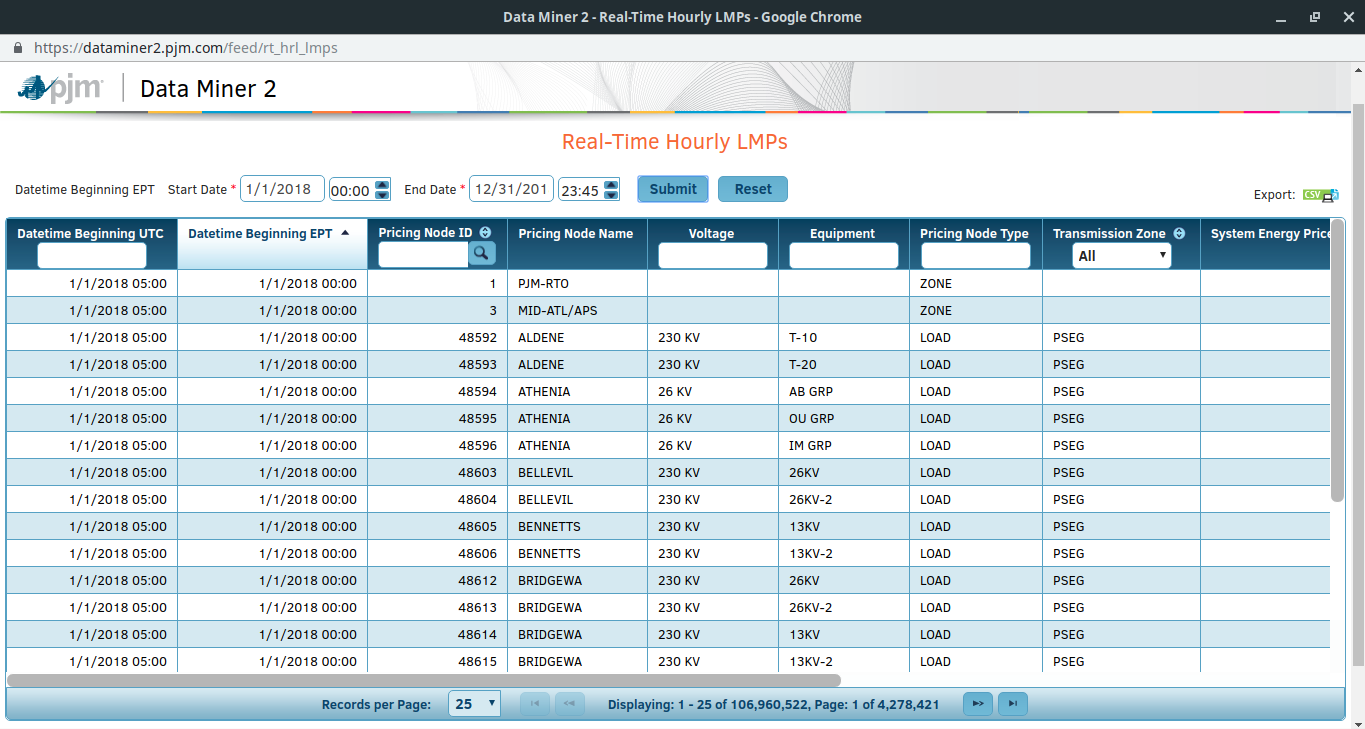
\includegraphics[scale=.3]{figuras/interface_dataminer.png}
	\end{center}
   \begin{center}
      \footnotesize {Fonte: \citeonline{interface2019pjm}}
   \end{center}
    \label{fig:interface_dataminer}
\end{figure}
\subsection{Escolha das ferramentas de programação}
Fez-se um estudo das ferramentas disponíveis no mercado para o problema em questão que se enquadra na categoria de \textit{data scraping} (técnica computacional na qual um programa extrai dados de saída legível somente para humanos, proveniente de um serviço ou aplicativo. Os dados extraídos geralmente são minerados e estruturados em um formato padrão como CSV, XML ou JSON).

Observando-se fatores como simplicidade, documentação das funcionalidades e custos, optou-se pela linguagem de programação JavaScript, mais especificamente pelo \textit{framework} Node.js. Sendo um dos \textit{frameworks} mais populares do mundo, permite resolver problemas robustos em poucas linhas de código, possui ampla documentação disponível e é gratuito (código-aberto).

Determinada a linguagem de programação, escolheu-se o editor de texto vscode por sua ampla adoção no mercado de desenvolvimento de software e sua grande gama de \textit{add-ons} que dão suporte ao desenvolvimento da linguagem JavaScript. Além disso, possui um terminal embutido que possibilita que os scripts sejam executado de dentro do próprio software.

Por fim, foram adotadas boas práticas de programação e ferramentas de \textit{source-control} foram escolhidas. A ferramente git unida com o gerenciador de repositórios Bitbucket mostraram-se suficientes para o projeto em questão.

\subsection{Extrator}
Os princípios que guiaram o desenvolvimento da ferramenta de extrair dados foram os de manter o código simples e limpo e fazê-lo de modo a ser reutilizável. Então os arquivos foram separados em funções e contam com comentários para facilitar o entendimento.

Para a adquirir os dados, usou-se o fato de o mercado em questão possuir uma \ac{API} \cite{api2019pjm}, que é uma interface que permite fazer aquisições diretamente com o banco de dados e que conta com mais recursos disponíveis. Além disso, cada aquisição passa a ser muito mais rápida, por justamente eliminar a necessidade de interagir com a interface web da aplicação. Para quantificar, uma aquisição manual que demorava 30 segundos para ser feita, agora pode ser feita em 2 segundos. 

Uma outra importante vantagem, está no fato de as aquisições poderem serem feitas de modo assíncrono, ou seja, é possível paralelizar o processo e deixá-lo ainda mais rápido. Por fim, vale mencionar o fato de que, uma vez que o controle do processo é feito de modo computacional, a probabilidade de equívocos ao fazer cada aquisição ou ao gravar e nomear os arquivos caem drasticamente.

Optou-se por baixar os dados no formato CSV, a razão principal é a versatilidade que esses tipos de arquivos possuem pois podem ser abertos em editores de texto ou em editores de planilha e já ficam visíveis de uma maneira inteligível.

No entanto, o formato CSV não é adequado para ser lido pelo AMPL, então há a necessidade de desenvolver uma solução que automatiza a conversão de cada arquivo gerado para o formato DAT, o qual pode ser lido pelo AMPL.

\subsection{Conversor}
O conversor desenvolvido, utilizando os mesmo recursos de programação usados no extrator, tem a tarefa de abrir cada arquivo CSV, separar apenas a coluna do preço da energia (Total LMP), e salvar de um modo específico no formato DAT, visto no apêndice \ref{apendice:exemplo.dat}, onde cada linha representa um índice e um parâmetro, que neste caso é o preço da energia a cada hora; desse modo, a leitura pelo AMPL seja otimizada. Uma peculiaridade é que o AMPL precisa pré-alocar memória para cada vetor de parâmetros, ou seja, é necessário saber de antemão o tamanho de cada vetor de entrada. Isso representa um problema pois nos vetores de entrada há tanto anos comuns como anos bissextos. A solução para isso foi registrar em cada arquivo o tamanho do vetor de parâmetros representado pelo símbolo tf.

\subsection{Código-fonte}
O código-fonte tanto do extrator como do conversor estão disponíveis nos apêndices \ref{apendice:extrator} e \ref{apendice:conversor}, respectivamente. No entanto, caso seja desejado executar o programa em questão, é recomendável seguir as boas práticas da programação e obter o código-fonte através do repositório online disponível em \cite{bitbucket}, pois assim é possível manter o código mais organizado, além de obter rapidamente as bibliotecas necessárias.

\section{Modelagem do envelhecimento da bateria aplicada ao AMPL}
\subsection{Estocagem de energia elétrica em baterias}
Estocagem de energia elétrica em bateria ou \ac{BESS} é um tema já presente há algumas décadas no mercado e conta com constantes avanços \cite{Doughty2010}. Dado que as curvas de demanda de energia geralmente possuem características marcantes, tanto horárias quanto sazonais como vistas nas figuras \ref{fig:dam2014} e \ref{fig:rtm2014}, o armazenamento através de baterias torna possível mitigar efeitos comuns decorrentes dessas curvas, ou seja, aumenta a oferta de energia em momentos de pico de consumo e permite estocar energia em momentos de baixa utilização, algo desejável e incentivado pelo operador do sistema elétrico. Além disso, também atrai investimentos pela possibilidade de lucro com a compra e venda, ou seja, arbitragem de energia no mercado livre.
%% FIGURA 3 - DAM
\begin{figure}[htb]
	\caption{Preço médio durante o dia do mercado do dia seguinte no ano de 2014.}
	\begin{center}
	    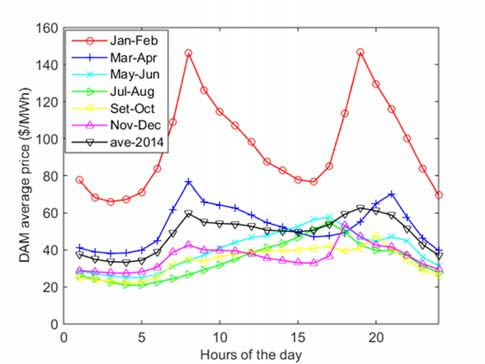
\includegraphics[scale=.6]{figuras/dam-hourly-2014.png}
	\end{center}
   \begin{center}
      \footnotesize {Fonte: \citeonline{Salles2016}}
   \end{center}
    \label{fig:dam2014}
\end{figure}
%% FIGURA 4 - RTM
\begin{figure}[htb]
	\caption{Preço médio durante o dia do mercado em tempo real no ano de 2014.}
	\begin{center}
	    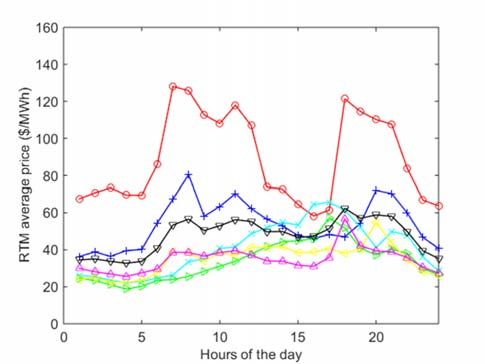
\includegraphics[scale=.6]{figuras/rtm-hourly-2014.png}
	\end{center}
   \begin{center}
      \footnotesize {Fonte: \citeonline{Salles2016}}
   \end{center}
    \label{fig:rtm2014}
\end{figure}

A partir dos avanços na tecnologia de estocagem, torna-se cada vez mais viável projetos de grande porte e consequente maior expressividade. A potência nominal eletroquímica instalada nos Estados Unidos vêm crescendo em ritmo acelerado no decorrer dos anos. Até 2015, haviam 14 unidades de armazenamento acima de 1MW no PJM \cite{Salles2016} enquanto que os dados até 2019 mostram 23 unidades na mesma faixa de potência \cite{doe2019}.
A crescente adoção desse modelo de estocagem de energia é justificada não só pelos benefícios citados ao sistema elétrico mas também pelo potencial de lucro a partir da operação no mercado livre. A partir da compra de energia elétrica mais barata em períodos de baixa demanda, estocagem e futura venda da energia por um preço maior em períodos de alta demanda.

\subsection{A tecnologia íons de lítio em baterias}
Baterias de íons de lítio foram propostas em meados de 1970 \cite{WHITTINGHAM1976} e desde então houve intenso desenvolvimento e melhorias nos quesitos de prolongamento da vida útil, aumento da densidade de carga, segurança, redução de custos e aumento da velocidade de carregamento \cite{Eftekhari2017}. Assim, atualmente, é vista como uma das tecnologia de armazenamento que mais crescem no mercado, devido a sua elevada densidade energética e sua eficiência próxima a 100\% \cite{michigan2018}.

Este trabalho abordará o modelo de bateria de lítio que descreve o processo de envelhecimento, que por sua vez está intrinsecamente ligado com a lucratividade do projeto. O desgaste da bateria decorre diretamente com a composição química bem como a rotina de operação da mesma. Alguns dos fatores ligados à degradação da bateria são: profundidade do descarregamento (\ac{DOD}), estado da carga (\ac{SOC}), temperatura (\textit{Temperature} ou T), taxa de carga e descarga (C-Rate) \cite{Wankmller2017}.

\subsection{Otimização considerando a degradação da bateria}
Considerando um cenário de operação da \ac{BESS} com previsão perfeita (\textit{perfect foresight}) do preço da energia a cada momento, é possível visualizar esta operação, que visa o máximo de lucro dado todas as limitações físicas apresentadas, como um problema de otimização. Desse modo, adota-se que a eficiência e os limites de carga e descarga da bateria como constantes e considera-se que o sistema esteja inserido no mercado norte-americano PJM. O equacionamento a ser otimizado será feito como visto em \cite{Wankmller2017} e descrito abaixo:

\subsection{Função Objetiva}
O máximo lucro é tido como:
\begin{equation}
    \label{eq:funcao_objetiva}
    max \sum_{t=1}^{T}{p}_{RT}[E_{V}(t) - E_{C}(t)] - \Delta{c}(t) 
\end{equation}
Onde $p_{RT}(t)$ é o preço da energia no instante t, $E_{V}(t)$ é a energia vendida, $E_{C}(t)$ é a energia comprada e $\Delta{c}(t)$ representa a penalidade da degradação da bateria, que será melhor abordada a seguir.

\subsection{Restrições do Modelo}
\label{constrains}
Existem limitações físicas e operacionais do modelo e serão equacionadas a seguir:

\begin{equation}
    \label{eq:constrain_1}
    SOC(t) = SOC_0 - E_{saindo}(t) + E_{entrando}(t), t = 1	
\end{equation}
\begin{equation}
    SOC(t) = SOC_{0}(t-1) - E_{saindo}(t) + E_{entrando}(t), t > 1 
\end{equation}

Onde $SOC(t)$ é o estado de carga após um período t, $SOC_0$ é a carga inicial e  $E_{saindo}(t)$,  $E_{entrando}(t)$ são as quantidades de energia descarregada e carregada, respectivamente.

    A máxima energia que pode entrar e sair da bateria é limitada pela máxima taxa de carregamento e descarregamento: $C_{car}$ e $C_{des}$ e a capacidade da bateria $Q_B$:
\begin{equation}
    E_{entrando}(t) \leq Q_B*1h*C_{car}*ID_{car}(t),\,\forall t
\end{equation}
\begin{equation}
    E_{saindo}(t) \leq Q_B*1h*C_{des}*ID_{des}(t),\,\forall t
\end{equation}

Onde $ID_{car}(t)$e $ID_{des}(t)$ são variáveis binárias, ou seja, apenas uma variável pode assumir valor 1, porém ambas as variáveis podem assumir valor 0, em todo e qualquer instante.
\begin{equation}
    ID_{car}(t) +ID_{des}(t) \leq 1,\,\forall t 
\end{equation}

 Desse modo, é modelado matematicamente o fato de a bateria estar hora carregando, hora descarregando.
 \begin{equation}
     E_c(t) - \frac{E_{entrando}(t)}{\eta_{entrando}},\,\forall t 
 \end{equation}
\begin{equation}
    E_v(t) - \frac{E_{saindo}(t)}{\eta_{saindo}},\,\forall t
\end{equation}

Onde $E_c(t)$e $E_v(t)$ são a quantidade de energia comprada e vendida no mercado num tempo específico t.

\begin{equation}
    SOC_{min} \leq SOC(t) \leq SOC_{max}(t),\,\forall t   
\end{equation}
O estado da corrente de carregamento respeita os limites acima.

\begin{equation}
    E_t(t) = E_{saindo}(t),\, t = 1
\end{equation}
\begin{equation}
    \label{eq:constrain_last}
    E_t(t) = E_t(t-1) + E_{saindo}(t),\, t > 1 
\end{equation}
Onde $E_t(t)$ é a energia total no momento t. As equação acima permitem manter registro da quantidade de energia descarregada a partir das baterias.

O modelo a ser otimizado é a função objetiva \ref{eq:funcao_objetiva} restringido pelas equações \ref{eq:constrain_1} a \ref{eq:constrain_last}. A modelagem matemática e resolução será feita pela ferramenta computacional AMPL munido, a princípio, do solucionador CPLEX.

\subsection{Cálculos da eficência da bateria}

A eficiência total de carga e descarga da bateria dependem das eficiência de carga e descarga e da eficiência de conversão de potência e do sistema de aquecimento/refrigeração:
\begin{equation}
    \eta_{entrando} = \frac{\eta_{sis} }{\eta_{car} }
\end{equation}

\begin{equation}
    \eta_{saindo} = \frac{\eta_{sis} }{\eta_{des} }
\end{equation}

As eficiências de carga e descarga da bateria dependem na tensão média de circuito aberto $U_{TCA}$ e da tensão média de carregamento/descarregamento ($V_{car}$ e $V_{des}$):
\begin{equation}
    \eta_{car} = \frac{V_{car} }{U_{TCA}}
\end{equation}
\begin{equation}
    \eta_{des} = \frac{V_{des} }{U_{TCA} }
\end{equation}

As tensões de carga e descarga podem ser representadas, respectivamente, por:
\begin{equation}
    V_{car} = U_{TCA} + I_{car}*R
\end{equation}
\begin{equation}
    V_{des} = U_{TCA} - I_{des}*R
\end{equation}
Onde R é a resistividade da bateria para operação contínua. E por fim a densidade de corrente de carga e descarga são, respectivamente:
\begin{equation}
    I_{car} = C_{car}*I
\end{equation}
\begin{equation}
    I_{des} = C_{des}*I
\end{equation}

Onde I é a densidade de corrente e $C_{car/des}$ é o C-rate da bateria.

\subsection{Modelo de Degradação}
O modelo de degradação elaborado irá restringir a operação da bateria de algumas maneiras, listadas a seguir e que serão argumentadas a na sequência:

 %\renewcommand{\labelenumi}{\Alph{enumi}}
 \begin{enumerate}
  \label{list:q_rem}
  \item A capacidade de armazenamento da bateria reduz de modo proporcional à energia total despachada pela mesma ao longo do tempo.
  \label{list:cp}
  \item A degradação da bateria entrará na estratégia de operação da mesma através de uma penalização de custo inserida na função objetiva.
   \label{list:SOC-range}
  \item O estado de carga \ac{SOC} máximo e mínimo serão ajustados de modo que a bateria opere em uma região linear de tensão.
\end{enumerate}

O embasamento teórico para \ref{list:q_rem} e \ref{list:q_rem} vem de um estudo encontrado em Watanabe et al. [24].
A princípio, será como base do estudo o mesmo modelo elaborado em \cite{Peterson2010} 
e adaptado no trabalho de \cite{Wankmller2017}:
\begin{equation}
    S_{rem}(t) = 1 - \frac{f_{DB}*E_{t}}{Q_{b}},\,\forall t 
\end{equation}

Onde $f_{DB}$ é uma constante de degradação da bateria estimada em $2,71*10^{-5}$.
%\section{Análise dos dados obtidos com ferramenta de \textit{business analytics}}
%\chapter[Resultados]{Resultados}
\label{resultados}

\chapter[Conclusões Parciais]{Conclusões Parciais}
\label{Conclusao}

Essa primeira etapa do projeto permitiu adquirir conceitos importantes, como noções sobre o funcionamento de um mercado livre de energia e sobre especificidades do funcionamento do PJM; contato com ferramentas de programação, com programação matemática, problemas de otimização e solucionadores comerciais.

A partir do estudo bibliográfico, foi possível entender em linhas gerais como um mercado funciona, suas siglas e os cálculos principais que são feitos para determinar o preço da energia. Além disso, foi possível ganhar conhecimentos específicos, como a possibilidade de existir energia com preço negativo, algo que inspira bastante a ideia de operar um \ac{BESS}.

O trabalho permitiu a ambientação com a forma como os dados eram adquiridos e mostrou-se que é possível automatizar essa tarefa através de ferramentas computacionais que permitem que tarefas iterativas sejam feitas de modo mais rápido e preciso.

De posse dos dados organizados e dispostos no formato DAT, foi possível ganhar noções de programação matemática através do \textit{software} AMPL. Assim, foram feitas otimizações como vistas em \cite{salles2017}, de modo a validar os dados adquiridos, consolidar essa etapa e permitir o início da aplicação das restrições equacionadas em \ref{constrains}.


Por fim, esse projeto permitiu o aprofundamento nos estudos relacionados a utilização de sistemas de armazenamento por meio de baterias operando em mercados livres de energia, sendo um estudo marcado pela adição do equacionamento do envelhecimento da bateria. Houve também importantes avanços na automatização no modo como os dados são adquiridos. Pode-se então colocar em prática os conhecimentos adquiridos nas diferentes matérias da graduação.



% ----------------------------------------------------------
% ELEMENTOS PÓS-TEXTUAIS
% ----------------------------------------------------------
\postextual

% ----------------------------------------------------------
% Referências bibliográficas
% ----------------------------------------------------------
\bibliography{bib/ref}

% ----------------------------------------------------------
% Glossário
% ----------------------------------------------------------
%
%\glossary

% ----------------------------------------------------------
% Apêndices
% ----------------------------------------------------------
% ---
% Inicia os apêndices
% ---
\begin{apendicesenv}
% Imprime uma página indicando o início dos apêndices
\partapendices

\appendix

\chapter[Scripts]{Scripts}
\label{scripts}

\lstset{style=}
\section{Algoritmo para definição dos nós}
\label{apendice:Algoritmo_nos.txt}
\lstinputlisting{apendices/Algoritmo_nos.txt}

\lstset{style=code}
\section{Exemplo de Arquivo DAT}
\label{apendice:exemplo.dat}
\lstinputlisting{apendices/exemplo.dat}

\section{Extrator de Dados} 
\label{apendice:extrator}
\lstinputlisting[language=JavaScript]{apendices/pjm-extrator.js}

\section{Conversor de CSV para DAT} 
\label{apendice:conversor}
\lstinputlisting[language=JavaScript]{apendices/from_csv_to_dat.js}



\end{apendicesenv}
% ---

% ----------------------------------------------------------
% Anexos
% ----------------------------------------------------------
% ---
% Inicia os anexos
% ---
%\begin{anexosenv}
% Imprime uma página indicando o início dos anexos
%\partanexos
% ---
% Incluir Anexo
% ---
%\chapter{Morbi ultrices rutrum lorem.}
%\lipsum[1-25]
%\section{Test}
%\lipsum[1-20]


%\end{anexosenv}


\end{document}


